\documentclass[12pt]{article}

\usepackage{graphicx}
\usepackage{amsmath}
\usepackage[margin=1in]{geometry}
\usepackage{fancyhdr}
\usepackage{enumerate}
\usepackage[shortlabels]{enumitem}
\usepackage[spanish]{babel}
\usepackage{xurl}
\usepackage{tcolorbox}
\usepackage{titlesec}
\usepackage{listings}
\usepackage{xcolor}

\titleclass{\subsubsubsection}{straight}[\subsection]

\newcounter{subsubsubsection}[subsubsection]
\renewcommand\thesubsubsubsection{\thesubsubsection.\arabic{subsubsubsection}}
\renewcommand\theparagraph{\thesubsubsubsection.\arabic{paragraph}} % optional; useful if paragraphs are to be numbered

\titleformat{\subsubsubsection}
  {\normalfont\normalsize\bfseries}{\thesubsubsubsection}{1em}{}
\titlespacing*{\subsubsubsection}
{0pt}{3.25ex plus 1ex minus .2ex}{1.5ex plus .2ex}

\makeatletter
\renewcommand\paragraph{\@startsection{paragraph}{5}{\z@}%
  {3.25ex \@plus1ex \@minus.2ex}%
  {-1em}%
  {\normalfont\normalsize\bfseries}}
\renewcommand\subparagraph{\@startsection{subparagraph}{6}{\parindent}%
  {3.25ex \@plus1ex \@minus .2ex}%
  {-1em}%
  {\normalfont\normalsize\bfseries}}
\def\toclevel@subsubsubsection{4}
\def\toclevel@paragraph{5}
%\def\toclevel@paragraph{6}
\def\toclevel@subparagraph{6}
\def\l@subsubsubsection{\@dottedtocline{4}{7em}{4em}}
\def\l@paragraph{\@dottedtocline{5}{10em}{5em}}
\def\l@subparagraph{\@dottedtocline{6}{14em}{6em}}
\makeatother

\setcounter{secnumdepth}{4}
\setcounter{tocdepth}{4}

% Set up headers and footers
\pagestyle{fancy}
\fancyhf{}  % Clear previous settings

\fancyhead[L]{Alvarado Ludwig - Vera Julián}
\fancyhead[C]{Simulación Estocástica}
\fancyhead[R]{9 de Marzo de 2025}

\fancyfoot[C]{\thepage}
\fancyfoot[C]{\footnotesize Este trabajo está bajo una licencia CC 4.0. Más info: \url{https://creativecommons.org/licenses/by/4.0/}}

\renewcommand{\headrulewidth}{0.2pt}

\lstdefinestyle{python}{
    language=Python,
    basicstyle=\ttfamily\footnotesize,
    keywordstyle=\color{blue}\bfseries,
    commentstyle=\color{gray},
    stringstyle=\color{red},
    numberstyle=\tiny\color{gray},
    numbers=left,
    stepnumber=1,
    frame=single,
    breaklines=true,
    tabsize=4,
    showstringspaces=false
}

\begin{document}

\tableofcontents


\section{\textit{Events and probability}}
\subsection{Punto a}
\subsubsection{Solución}

Se considera una caja con tres canicas de colores rojo, verde y ayuzal como la de la figura \ref{fig:caja-canica}, nos dicen que en el experimento se toma una canica y despues se vuelve a poner en la caja, es decir, si definimos los eventos como:

\begin{itemize}
  \item \(A\) sacar canica verde.
  \item \(B\) sacar canica azul.
  \item \(C\) sacar canica roja.
\end{itemize}

Se afirma que los eventos \(A, B\) y \(C\) son independientes los unos de los otros, ya que, estos no dependen del otro.

\begin{itemize}
  \item \textbf{Espacio muestral (\(\Omega\)):} de acuerdo a la definición ``Es el conjunto de todos los posibles resultados de un experimento aleatorio.'' En este experimento solo se pueden tener diferentes pares de resultados Por lo tanto, la combinación de estos resultados da como resultado el siguiente conjunto:
        \[
        \Omega = \{ (A,A), (A, B), (A, C), (B, A), (B, B), (B, C), (C, A), (C, B), (C, C)  \}
        \]
  Al sacar \(|\Omega|\) este resultado es de \(9\) posibles resultados del experimento. 
  \item \textbf{Probabilidad de cada canica:} el enunciado nos dice que cada canica tiene el mismo chance de ser seleccionada, es decir, una entre tres canicas, por lo tanto, las probabilidades de cada evento se definen como:
        \[
        P(A) = \frac{1}{3} = 0.33\overline{333} \qquad P(B) = \frac{1}{3} = 0.33\overline{333} \qquad P(C) = \frac{1}{3} = 0.33\overline{333}
        \]
        Las dos sacadas son independientes, por lo tanto, se puede aplicar que para cada par \((X, Y)\) se cumpla:
        \[
        P(X) \times P(Y) = \frac{1}{3} \times \frac{1}{3} = \frac{1}{9} = 0.11\overline{111}
        \]
        Por lo tanto, cada punto en el espacio muestral es de \(\frac{1}{9}\).
\end{itemize}



\begin{figure}[ht]
  \centering
  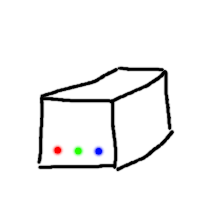
\includegraphics[width=0.4\textwidth]{img/Caja.png}
  \caption{\label{fig:caja-canica} Caja con 3 canicas de colores rojo, verde y azul. Ilustración de los autores elaborada en el software GIMP.}
\end{figure}


\subsection{Punto b}
\subsubsection{Solución}

En este punto nos plantean la misma situación anterior pero los eventos son \textbf{dependientes}, ya que, se saca la primera canica y no se vuelve a meter, es decir, si saco la canica azul como se ve en la figura \ref{fig:caja-2} para la segunda sacada de canica la probabilidad no va a ser la misma, puesto que, hay únicamente dos canicas a sacar. 

\begin{figure}[ht]
  \centering
  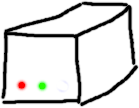
\includegraphics[width=.3\textwidth]{img/Caja2.png}
  \caption{\label{fig:caja-2} Caja con canicas verde y roja. Ilustración de los autores elaborada en el software GIMP.}
\end{figure}


Entonces, el conjunto del espacio muestral \(\Omega\) queda como:

\[
  \Omega = \{ (A, B), (A, C), (B, A), (B, C), (C, A), (C, B)\}
\]

La cardinalidad entonces del conjunto \(\Omega\) es de 6.

Teniendo en cuenta la probabilidad para dos eventos dependientes:

\[
P(X \cap Y) = P(X|Y) P(Y)
\]

Si sacamos una canica de color rojo (\(P(C)\)) su probabilidad se mantiene como la del mundo anterior \(\frac{1}{3}\). Podemos deducir que en el espacio muestral quedan las canicas azul y verde, si deseamos sacar la azul \((P(B)\), esta está condicionada por el evento anterior de sacar la roja. Teniendo en cuenta, lo anterior, la probabilidad de sacar una canica azul será \(P(B|C) = \frac{1}{2}\). Por lo tanto, al realizar la operación:

\[
 P(B|C)P(C) = \frac{1}{2} \times \frac{1}{3} = \frac{1}{6} = 0.166\overline{666}
\]

Generalizando con \((X, Y)\) siendo un par del espacio muestral \(\Omega\):

\[
P(X \cap Y) = P(X|Y)P(Y) = \frac{1}{2} \times \frac{1}{3} = \frac{1}{6} =  0.166\overline{666}
\]

En conclusión, la probabilidad para cada canica dado que se saque una antes y no se vuelva a introducir es de \(0.166\overline{666}\). 

\section{\textit{Congruential generators}}
\subsection{Solución}

Teniendo en cuenta:

\[
X_{n} = (9X_{n-1} + 3) \mod 11
\]






\section{\textit{Uniformity and independence of the unif}}
\subsection{Solución}

\section{\textit{Inverse method for a discrete r.v}}

\subsection{Punto a}
\subsection{Solución}

\subsection{Punto b}
\subsection{Solución}

\subsection{Punto c}
\subsection{Solución}

\subsection{Punto d}
\subsection{Solución}

\subsection{Punto e}
\subsection{Solución}

\subsection{Punto f}
\subsection{Solución}


\section{\textit{Inverse method for continuos r.v}}

\subsection{Punto a}
\subsection{Solución}

\subsection{Punto b}
\subsection{Solución}

\subsection{Punto c}
\subsection{Solución}

\subsection{Punto d}
\subsection{Solución}

\subsection{Punto e}
\subsection{Solución}


\section{\textit{Monte Carlo Integration}}
\subsection{Solución}

\section{\textit{Estimating} \(\pi\)}

\subsection{Punto a}
\subsection{Solución}

\subsection{Punto b}
\subsection{Solución}

\subsection{Punto c}
\subsection{Solución}

\subsection{Punto d}
\subsection{Solución}

\subsection{Punto e}
\subsection{Solución}



\section{\textit{Estimating expected values with Monte Carlo} \(\pi\)}

\subsection{Punto a}
\subsection{Solución}

\subsection{Punto b}
\subsection{Solución}

\subsection{Punto c}
\subsection{Solución}

\subsection{Punto d}
\subsection{Solución}

\subsection{Punto e}
\subsection{Solución}


\end{document}
